\section{Analysis: Why DHCD is Saturated}
\label{sec:analysis}

\subsection{The Shared Error Floor}

DHCD now has a shared error floor, not just hard examples: across all 15
\modelname{} students and the reproduced baseline~\cite{malla2025},
\textbf{11 images} defeat every model.  \emph{No} configuration classifies
these samples correctly, regardless of architecture, training strategy, or
random seed.

\begin{figure}[t]
  \centering
  \begin{subfigure}[t]{0.48\linewidth}
    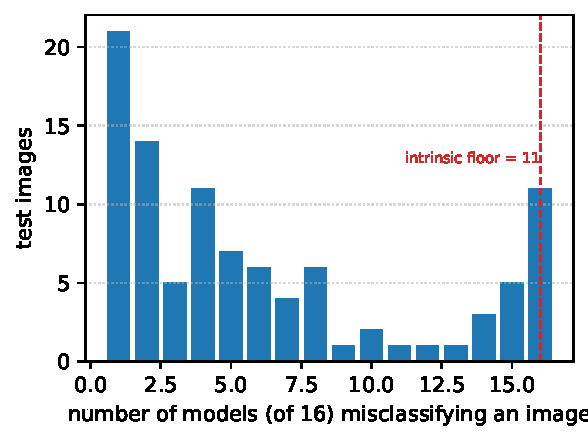
\includegraphics[width=\linewidth]{figures/error_floor.pdf}
    \caption{Images missed by exactly $k$ of the 16 models.
      Eleven are missed by all 16 simultaneously---an irreducible floor.}
    \label{fig:floor}
  \end{subfigure}\hfill
  \begin{subfigure}[t]{0.48\linewidth}
    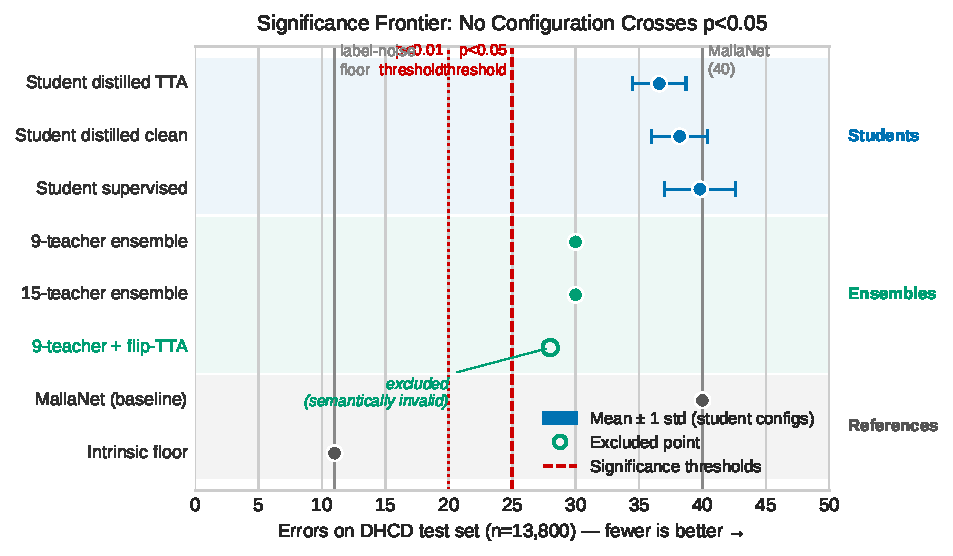
\includegraphics[width=\linewidth]{figures/significance_frontier.pdf}
    \caption{Every configuration sits above the $p{<}0.05$ threshold
      (25 errors). The 11-error floor marks the hard lower bound.}
    \label{fig:sig-frontier}
  \end{subfigure}
  \caption{Left: shared error floor across all 16 models.
    Right: significance frontier---30-error clean ensemble and 36.6-error
    student mean both lie in the statistical parity region.}
\end{figure}

When the same 11-image floor catches both a 1.11\,M-parameter compact
student and a baseline fifteen times its size, the problem is in the data.
Outside this floor, errors are model-specific (mean pairwise Jaccard
similarity $\mathbf{0.48}$): seeds shuffle which images fail, but
ensembling or adding seeds reduces \emph{variance}, not the \emph{bias} the
floor imposes.

\subsection{Confusable Character Pairs}

Script-level collisions dominate remaining mistakes.  Table~\ref{tab:confusions} lists
the top distilled-student confusion pairs aggregated across the 10
distilled seeds.  \textbf{ba / waw} leads with 17 cross-confusions, followed by
\textbf{waw / tabala} (16) and \textbf{tra / ba} (15); \textbf{dha / gha}
(13 instances) and \textbf{da / dhaa} (9 instances) round out the top five.

\begin{table}[t]\centering
\caption{Top confusion pairs in the distilled student pool (aggregate
  across 10 distilled seeds on the DHCD test set).}
\label{tab:confusions}
\begin{tabular}{lcc}\toprule
Pair & Cross-confusions & Script note \\\midrule
ba $\leftrightarrow$ waw    & 17 & Near-identical body, open vs.\ closed loop \\
waw $\leftrightarrow$ tabala & 16 & Shared curved baseline \\
tra $\leftrightarrow$ ba    & 15 & Conjunct ligature vs.\ simple consonant \\
dha $\leftrightarrow$ gha   & 13 & Looped ascender, subtle body curvature \\
da $\leftrightarrow$ dhaa   & 9  & Single hairline distinguishes the pair \\\bottomrule
\end{tabular}
\end{table}

These pairs expose a resolution limit: the confusable glyphs differ by
strokes finer than a few pixels at $32{\times}32$ resolution, and DHCD
provides neither higher-resolution inputs nor stroke-level annotation.

\subsection{Significance Frontier}
\label{sec:sig-frontier}

Under the exact two-sided McNemar test~\cite{mcnemar1947} at $\alpha = 0.05$,
crossing from statistical parity to a demonstrable improvement over the
reproduced baseline (40 errors) requires at most \textbf{25 errors}
($\geq$99.82\% accuracy) --- fewer than 15 additional correct classifications
separating inconclusive from significant.  A comfortable margin would require
$\leq$\textbf{20 errors} ($\geq$99.855\%), a target that demands
near-perfect resolution of the ambiguous-glyph pairs in
Table~\ref{tab:confusions}.

Every configuration tested stops just short of this frontier.  The best
single result is \textbf{28 errors}: the 9-teacher ensemble with
(semantically invalid) flip-TTA applied at test time, a result excluded
on methodological grounds (Section~\ref{sec:flip-tta}).  The best
defensible single seed reaches \textbf{34 errors}; the best ensemble
without flip-TTA reaches \textbf{30 errors}.  Both sit within the parity
region, separated from significance by the 11-image irreducible floor itself.

\textbf{No lever tested in this study achieved a statistically
significant improvement over the baseline.}  Scaling the teacher pool from 9
to 15, applying TTA-softened distillation targets, and running five
independent seeds all leave configurations outside the significance
frontier.  This is not a failure of experimental design---it defines a
saturated benchmark.  The significance frontier is not a line researchers
are approaching asymptotically, but a wall built from mislabelled images
and inherently ambiguous glyphs.


\subsection{Calibration}

Expected Calibration Error (ECE)~\cite{guo2017calibration} falls in the
range \textbf{0.13--0.16} across all \modelname{} configurations ---
unremarkable values for softmax classifiers without post-hoc temperature
scaling.  ECE does not co-vary with accuracy across seeds: better seeds are
not better calibrated.  Critically, the 11 floor images are confidently
wrong, not uncertain: models assign high probability to an incorrect class
on every seed, confirming the error floor is a data-level property that
architectural or training choices cannot correct.
